\chapter{Endocrinologie en homeostase}\label{ch:b3:endocrinology}

In de zomer van 1921 bonden twee jonge mannen in een heet laboratorium
in Toronto de afvoerbuizen van de alvleesklier van honden af, wachtten
tot het verteringsweefsel was verschrompeld, vermaalden wat er over was
en spoten het extract in bij een hond die door het wegnemen van zijn
alvleesklier suikerziek was gemaakt. Zijn bloedsuiker daalde. In
januari kreeg een veertienjarige jongen die in het Toronto General
Hospital aan suikerziekte lag te sterven het extract, en binnen enkele
weken at hij, liep hij en kwam hij aan; hij leefde nog dertien jaar. De
stof, \omterm{def:b3:endocrinology:glucose}{insuline}, is een peptide van eenenvijftig aminozuren dat door een
procent van de alvleesklier in het bloed wordt uitgescheiden, waar het
bij een concentratie van enkele honderden picomol per liter aan elke
spier- en vetcel van het lichaam vertelt wat het met de suiker van de
laatste maaltijd moet doen. Dit hoofdstuk gaat over zulke
boodschappers: wat zij zijn, hoe een cel die de klier nooit heeft
ontmoet weet wat de boodschap betekent, hoe de klieren zelf in een
hiërarchie van terugkoppelingen worden bestuurd, en hoe het hele
stelsel de glucose, het zout, het calcium en de temperatuur van het
bloed een leven lang binnen enkele procenten houdt --- en wat er in de
kliniek gebeurt wanneer een van de lussen faalt.

\section{Hormonen en hun receptoren}

\begin{definition}[Hormoon]\label{def:b3:endocrinology:hormone}
\index{hormoon}\index{endocriene klier}\index{paracrien}\index{steroïdhormoon}\index{peptidehormoon}\index{kernreceptor}
Een \emph{hormoon} is een stof die een cel in het bloed afgeeft en die
werkt op verre cellen die de receptor ervoor dragen; een
\emph{paracrien} signaal werkt op de buren, een \emph{autocrien} op de
cel die het maakte, en een neurohormoon wordt door een neuron in het
bloed afgegeven. De klassieke \emph{endocriene klieren} --- \omterm{def:b3:endocrinology:axes}{hypofyse},
schildklier, bijschildklieren, bijnieren, eilandjes van de
alvleesklier, geslachtsklieren --- hebben gezelschap gekregen van het
hart (natriuretisch peptide), de nier (erytropoëtine), het vet
(leptine), de darm (een dozijn peptiden) en het bot. Chemisch zijn
hormonen van drie soorten, en de chemie legt het mechanisme vast.
\emph{Peptide- en eiwithormonen} (\omterm{def:b3:endocrinology:glucose}{insuline}, groeihormoon, de hormonen
van de \omterm{def:b3:endocrinology:axes}{hypofyse}) worden op ribosomen gemaakt, in korrels opgeslagen,
door exocytose afgegeven, reizen vrij in het plasma, kunnen geen
membraan passeren en werken op receptoren aan het celoppervlak ---
gekoppeld aan een G-eiwit of aan een kinase --- via tweede
boodschappers, binnen seconden tot minuten; hun halveringstijden zijn
minuten. \emph{Steroïden} (cortisol, \omterm{def:b3:renal-osmoregulation:controls}{aldosteron}, oestrogenen,
testosteron, en het secosteroïde \omterm{def:b3:endocrinology:calcium}{vitamine D}) worden naar behoefte uit
cholesterol gemaakt, niet opgeslagen, reizen gebonden aan
transporteiwitten, gaan door membranen heen en binden
\emph{kernreceptoren} die zelf transcriptiefactoren zijn: hun werking
kost uren en houdt dagen aan. \emph{Aminen} staan tussen beide in:
adrenaline werkt binnen een seconde aan het oppervlak; de
schildklierhormonen werken, hoewel afgeleid van een aminozuur, als
steroïden op kernreceptoren. Een hormoon betekent op zichzelf niets:
dezelfde adrenaline verwijdt het ene vat en vernauwt het andere omdat
hun gladde spieren verschillende receptorsubtypen dragen, en hetzelfde
cortisol verhoogt de bloedglucose in de lever en onderdrukt een
\omterm{def:b3:adaptive-immunity:lymphocytes}{lymfocyt} omdat het \omterm{def:b3:chromatin-epigenetics:nucleosome}{chromatine} van de twee cellen zijn receptor
verschillende genen aanbiedt.
\end{definition}

\begin{omfigure}
\begin{tikzpicture}[every node/.style={font=\scriptsize}, >=stealth]
  % peptide pathway
  \draw[thick, omDef, fill=omDef!10] (0,0) rectangle (5.2,3.4);
  \node[above] at (2.6,3.4) {peptide- of aminehormoon --- receptor aan het oppervlak};
  \draw[thick, omDef] (0,2.6) -- (5.2,2.6); \node[left, font=\tiny] at (5.2,2.75) {membraan};
  \node[circle, fill=omThm!60, inner sep=2pt, label={[font=\tiny]right:hormoon}] (h1) at (1.4,3.1) {};
  \draw[thick, omDef!80!black, fill=omDef!40] (1.1,2.3) rectangle (1.7,2.9); \node[below, font=\tiny] at (1.4,2.3) {receptor};
  \draw[->, thick] (2.0,2.1) -- (3.0,2.1) node[right, align=left, font=\tiny] {G-eiwit of\\kinaseactiviteit};
  \draw[->, thick] (2.6,1.75) -- (2.6,1.25) node[below, align=center, font=\tiny] {cAMP, Ca$^{2+}$, IP$_3$ of\\fosforyleringscascade};
  \draw[->, thick] (2.6,0.55) -- (2.6,0.25) node[below=-2pt, font=\tiny] {enzymen omgeschakeld: seconden tot minuten};
  % steroid pathway
  \draw[thick, omProp, fill=omProp!10] (6.4,0) rectangle (11.6,3.4);
  \node[above] at (9.0,3.4) {steroïd- of schildklierhormoon --- kernreceptor};
  \draw[thick, omProp] (6.4,2.6) -- (11.6,2.6);
  \node[circle, fill=omMeth!70, inner sep=2pt, label={[font=\tiny]right:hormoon op transporteiwit}] (h2) at (7.6,3.1) {};
  \draw[->, thick] (7.6,2.95) -- (7.6,2.2) node[below, font=\tiny] {diffundeert erdoorheen};
  \draw[->, thick] (7.9,1.85) -- (9.0,1.5); \draw[thick, omProp!80!black, fill=omProp!35] (8.8,1.0) rectangle (9.6,1.7); \node[right, align=left, font=\tiny] at (9.65,1.35) {hormoon--receptor-\\complex, een\\transcriptiefactor};
  \draw[thick, omProp] (7.0,0.2) rectangle (11.0,0.8); \node[font=\tiny] at (9.0,0.5) {kern: genen aan of uit --- uren tot dagen};
  \draw[->, thick] (9.2,1.0) -- (9.2,0.82);
\end{tikzpicture}

{\small Twee manieren om een \omterm{def:b3:endocrinology:hormone}{hormoon} te horen. Wateroplosbare \omterm{def:b3:endocrinology:hormone}{hormonen}
blijven aan het oppervlak staan en werken via tweede boodschappers,
snel en kort; vetoplosbare gaan naar binnen, binden een receptor die
een transcriptiefactor is, en veranderen wat de cel maakt, traag en
voor lang.}
\end{omfigure}

\begin{proposition}[Dosis en antwoord]\label{prop:b3:endocrinology:dose}
\index{dosis--antwoordkromme}\index{reservereceptoren}\index{neerregulatie}
Een cel met $R$ receptoren met dissociatieconstante $K_{d}$ heeft bij
een hormoonconcentratie $H$ er $R\,H/(K_{d} + H)$ van bezet, en het
antwoord stijgt gewoonlijk met de bezetting langs een sigmoïde op een
logaritmische dosis-as, half maximaal bij een $\text{EC}_{50}$ die vaak
ver onder $K_{d}$ ligt: enkele procenten bezetting geven al een vol
antwoord, omdat het signaal stroomafwaarts wordt versterkt (één
receptor activeert vele G-eiwitten, één kinase fosforyleert vele
substraten), en de overtollige \emph{\omterm{prop:b3:endocrinology:dose}{reservereceptoren}} verschuiven de
kromme naar links en maken de cel gevoelig voor lage doses. De cel
stemt haar eigen gevoeligheid af: langdurige blootstelling aan een
\omterm{def:b3:endocrinology:hormone}{hormoon} haalt de receptoren ervoor van het oppervlak weg
(\emph{neerregulatie}), het mechanisme waardoor een aanhoudend hoge
\omterm{def:b3:endocrinology:glucose}{insuline} de werking van \omterm{def:b3:endocrinology:glucose}{insuline} zelf afstompt; onthouding vermeerdert
ze. \omterm{def:b3:endocrinology:hormone}{Hormonen} circuleren bij $10^{-12}$ tot $10^{-9}$ molair --- duizend
tot een miljoen maal onder de meeste metabolieten --- en daarom moeten
receptoren ze met nanomolaire affiniteit binden, en daarom was er voor
het meten ervan een nieuwe methode nodig.
\end{proposition}
\begin{proof}
De bezetting is de isotherm van de massawerking van één bindingsplaats.
Verzadigt het antwoord al wanneer $n \ll R$ receptoren bezet zijn, dan
is het half maximaal wanneer $R H/(K_{d} + H) = n/2$, d.w.z.\ $H = K_{d}\,
(n/2)/(R - n/2) \approx K_{d}\, n/(2R) \ll K_{d}$: de EC$_{50}$ daalt
evenredig met de overmaat aan receptoren. Receptoren verliezen verhoogt
haar, en dat is het effect van de neerregulatie op de kromme.
\end{proof}

\begin{method}[Radio-immunoassay]\label{met:b3:endocrinology:ria}
\index{radio-immunoassay}\index{immunoassay}
Om een \omterm{def:b3:endocrinology:hormone}{hormoon} bij een concentratie van picomol per liter te meten
(Yalow en Berson, 1959): (1) wek een \omterm{def:b3:adaptive-immunity:antibody}{antilichaam} ertegen op; (2) meng
een vaste kleine hoeveelheid \omterm{def:b3:adaptive-immunity:antibody}{antilichaam} met een vaste hoeveelheid
radioactief gemerkt \omterm{def:b3:endocrinology:hormone}{hormoon}, en voeg het monster toe; (3) het
ongemerkte \omterm{def:b3:endocrinology:hormone}{hormoon} van het monster wedijvert met het gemerkte om de
plaatsen van het \omterm{def:b3:adaptive-immunity:antibody}{antilichaam}, dus hoe meer \omterm{def:b3:endocrinology:hormone}{hormoon} het monster bevat,
hoe minder merkstof er wordt gebonden; (4) scheid gebonden van vrije
merkstof en tel; (5) lees de concentratie van het monster af op een
ijkkromme die met bekende hoeveelheden is gemaakt. De nakomelingen
ervan vervangen de isotoop door een enzym of een fluorofoor en
gebruiken twee antilichamen (een ``sandwich'') om specificiteit te
winnen; zij meten elk \omterm{def:b3:endocrinology:hormone}{hormoon} van dit hoofdstuk uit een druppel bloed,
en hebben van de endocrinologie een kwantitatieve wetenschap gemaakt.
\end{method}

\section{De hiërarchie: hypothalamus en hypofyse}

\begin{definition}[De assen]\label{def:b3:endocrinology:axes}
\index{hypothalamus}\index{hypofyse}\index{poortadersysteem}\index{vrijmakend hormoon}\index{troop hormoon}\index{negatieve terugkoppeling}
De \emph{hypothalamus}, enkele grammen brein boven de hypofyse, zet
neurale informatie --- stress, koude, daglengte, de \omterm{def:b3:renal-osmoregulation:problem}{osmolariteit} en de
glucose van het bloed --- om in hormonale bevelen. Zijn
neurosecretoire cellen geven \emph{vrijmakende \omterm{def:b3:endocrinology:hormone}{hormonen}} af (peptiden:
CRH, TRH, GnRH, GHRH, en de remmer somatostatine; dopamine voor
prolactine) aan een eigen \emph{poortadersysteem} van vaten dat ze
onverdund een centimeter omlaag draagt naar de \emph{voorkwab van de
hypofyse}, wier cellen antwoorden met \emph{trope \omterm{def:b3:endocrinology:hormone}{hormonen}}: ACTH naar
de bijnierschors, TSH naar de schildklier, LH en FSH naar de
geslachtsklieren, groeihormoon naar de lever en de weefsels,
prolactine naar de borst. De \omterm{def:b3:endocrinology:hormone}{hormonen} van de doelklieren --- cortisol,
thyroxine, geslachtssteroïden --- koppelen terug op zowel de hypofyse
als de hypothalamus om hun eigen bevelen af te zetten:
\emph{negatieve terugkoppeling}, in drie lagen. De \emph{achterkwab van
de hypofyse} is geen klier maar bestaat uit de axonuiteinden van
neuronen van de hypothalamus, die vasopressine en oxytocine
rechtstreeks in het bloed afgeven. Elke as heeft haar eigen dynamiek:
de schildklieras is traag en gestaag en houdt een \omterm{thm:b3:endocrinology:loop}{instelpunt} jarenlang
vast; de bijnieras is pulserend en circadiaan, met een piek van
cortisol vóór de dageraad en afgifte in salvo's per uur; de
geslachtsas van een vrouw draait een maandelijkse cyclus op een
positieve terugkoppeling die de andere missen.
\end{definition}

\begin{omfigure}
\begin{tikzpicture}[every node/.style={font=\scriptsize}, >=stealth]
  \node[draw, thick, rounded corners, fill=omDef!20, align=center, minimum width=3.2cm] (hyp) at (0,3.4) {hypothalamus\\CRH, TRH, GnRH, GHRH};
  \node[draw, thick, rounded corners, fill=omDef!20, align=center, minimum width=3.2cm] (pit) at (0,1.7) {voorkwab hypofyse\\ACTH, TSH, LH/FSH, GH};
  \node[draw, thick, rounded corners, fill=omProp!25, align=center, minimum width=3.2cm] (gl) at (0,0) {doelklier\\cortisol, T$_4$, geslachtssteroïden};
  \node[draw, thick, rounded corners, fill=omMeth!25, align=center, minimum width=3.2cm] (tis) at (0,-1.7) {weefsels: effecten};
  \draw[->, very thick] (hyp) -- (pit) node[midway, right, font=\tiny] {poortadervaten};
  \draw[->, very thick] (pit) -- (gl) node[midway, right, font=\tiny] {bloed};
  \draw[->, very thick] (gl) -- (tis);
  \draw[-|, thick, omThm] (gl.west) -- ++(-0.9,0) |- (pit.west) node[pos=0.25, left, font=\tiny, omThm, align=right] {korte\\lus};
  \draw[-|, thick, omThm] (gl.west) ++(-0.9,0) -- ++(-0.7,0) |- (hyp.west) node[pos=0.25, left, font=\tiny, omThm, align=right] {lange\\lus};
  \node[left, align=right, font=\tiny] at (-2.0,4.4) {invoer: stress, koude,\\licht, metabolieten};
  \draw[->, thick] (-1.9,4.3) -- (hyp.north west);
  % right: the thyroid example with numbers
  \node[right, align=left] at (3.4,3.4) {schildklieras: TRH $\to$ TSH $\to$ T$_4$, T$_3$;\\halveringstijd T$_4$ 7 dagen, instelpunt jarenlang vast;\\log TSH daalt lineair als vrij T$_4$ stijgt};
  \node[right, align=left] at (3.4,1.7) {bijnieras: CRH $\to$ ACTH $\to$ cortisol;\\pulsen elke 1--2 h, piek vóór het ontwaken;\\stress overstemt de terugkoppeling};
  \node[right, align=left] at (3.4,0) {geslachtsas: GnRH-pulsen $\to$ LH, FSH $\to$\\oestradiol, progesteron, testosteron;\\eens per maand een golf door positieve terugkoppeling};
  \node[right, align=left] at (3.4,-1.7) {groeias: GHRH, somatostatine $\to$ GH $\to$\\IGF-1 uit de lever; pulsen 's nachts};
\end{tikzpicture}

{\small De assen met drie lagen. Vrijmakende \omterm{def:b3:endocrinology:hormone}{hormonen} bereiken de
\omterm{def:b3:endocrinology:axes}{hypofyse} door de poortadervaten; de \omterm{def:b3:endocrinology:axes}{hypofyse} beveelt een klier; het
\omterm{def:b3:endocrinology:hormone}{hormoon} van de klier zet beide lagen stroomopwaarts af. Elke as heeft
haar eigen ritme en haar eigen tekortkomingen.}
\end{omfigure}

\begin{proof}[Bewijsmateriaal]
Berthold (1849) castreerde jonge hanen, die hun kam, hun kraai en hun
strijdlust verloren; een teelbal ergens in de buik terugplaatsen,
zonder zijn zenuwen, gaf ze terug --- het orgaan werkte via het bloed.
Harris (jaren 1950) sneed bij ratten de poortadervaten tussen
\omterm{def:b3:endocrinology:axes}{hypothalamus} en \omterm{def:b3:endocrinology:axes}{hypofyse} door: de \omterm{def:b3:endocrinology:axes}{hypofyse}, wier bloedtoevoer van
elders was hersteld, antwoordde niet meer op stress en de eierstokken
hielden op te cycleren; een \omterm{def:b3:endocrinology:axes}{hypofyse} onder de nier verplant bleef
inert, maar onder de \omterm{def:b3:endocrinology:axes}{hypothalamus}, waar er poortadervaten in
teruggroeiden, werkte zij --- het brein bestuurt de klier met stoffen
uit het bloed, en Guillemin en Schally isoleerden daarna de eerste
ervan, TRH, uit miljoenen hypothalami van schapen en varkens (1969):
drie aminozuren.
\end{proof}

\begin{proposition}[Terugkoppeling en de log-lineaire schildklier]\label{prop:b3:endocrinology:thyroid}
\index{schildklierhormoon}\index{TSH}\index{hypothyreoïdie}\index{hyperthyreoïdie}\index{struma}
De schildklier neemt jodide op en maakt thyroxine T$_{4}$ (vier
jodiumatomen), dat de weefsels omzetten in het werkzame T$_{3}$; beide
verhogen de stofwisseling van bijna elke cel, bepalen de hartslag en
zijn nodig voor de ontwikkeling van het brein vóór en na de geboorte.
TSH uit de \omterm{def:b3:endocrinology:axes}{hypofyse} drijft zowel de aanmaak als de groei van de klier
aan; T$_{4}$ onderdrukt TSH. Het verband in de stationaire toestand is
\emph{log-lineair}: de logaritme van TSH daalt evenredig met het vrije
T$_{4}$,
\[
\text{TSH} = \text{TSH}_{0}\,\mathrm{e}^{-\kappa\,(T_{4} - T_{4,0})},
\]
zodat een daling van het vrije T$_{4}$ met een derde de TSH ongeveer
tienvoudig verhoogt --- en daarom is TSH, en niet T$_{4}$, de gevoelige
bepaling: een klier die begint te falen toont een normaal T$_{4}$ dat
door een reeds enkele malen verhoogde TSH op peil wordt gehouden. Falen
van de klier (auto-immuunvernietiging, jodiumgebrek) geeft
\emph{hypothyreoïdie} --- koud, traag, moe, met een hoge TSH en, bij
jodiumgebrek, een klier die door de TSH die haar niet aan het
produceren krijgt tot een \emph{struma} is uitgezet; een \omterm{def:b3:adaptive-immunity:antibody}{antilichaam}
dat TSH nabootst geeft \emph{hyperthyreoïdie} (de ziekte van Graves)
met een warme, snelle, magere patiënt en een TSH die tot niets is
onderdrukt, omdat de prikkeling aan de terugkoppeling ontsnapt. Een
pasgeborene zonder \omterm{prop:b3:endocrinology:thyroid}{schildklierhormoon} ontwikkelt binnen maanden een
onomkeerbare verstandelijke beperking, en daarom wordt bij elke
pasgeborene de TSH in een druppel bloed gemeten.
\end{proposition}
\begin{proof}
De TSH-afgifte van de cel in de \omterm{def:b3:endocrinology:axes}{hypofyse} antwoordt op de bezetting van
de receptor door T$_{3}$, dat zelf evenredig is met T$_{4}$, en het
antwoord van een transcriptionele onderdrukking op een verandering in
de bezetting is multiplicatief --- elke toename van het \omterm{def:b3:endocrinology:hormone}{hormoon}
onderdrukt dezelfde fractie van wat er over is --- dus
$\mathrm{d}\ln\text{TSH}/\mathrm{d}T_{4} = -\kappa$, waaruit de
exponentiële vorm volgt. Met $\kappa$ zo gefit dat $T_{4}$ dat daalt
van $15$ naar \qty{10}{pmol/L} de TSH van $1.5$ naar \qty{15}{mU/L}
verhoogt, is $\kappa = \ln 10/5 = \qty{0.46}{L/pmol}$: de TSH verdubbelt
voor elke \qty{1.5}{pmol/L} T$_{4}$ die verloren gaat, en dat is de
versterking die er de gevoelige bepaling van maakt.
\end{proof}

\begin{omfigure}
\begin{tikzpicture}
\begin{semilogyaxis}[
  width=0.6\linewidth, height=5.6cm,
  axis x line=bottom, axis y line=left,
  xmin=4, xmax=30, ymin=0.02, ymax=200,
  xlabel={vrij T$_4$ (pmol/L)}, ylabel={TSH (mU/L)},
  xlabel style={font=\small, at={(axis description cs:0.5,-0.12)}, anchor=north}, ylabel style={font=\small},
  tick label style={font=\small}, xtick={5,10,15,20,25,30}, ytick={0.1,1,10,100},
  yticklabels={0.1,1,10,100},
  clip=false,
]
\addplot[very thick, omDef, domain=4.5:24.4, samples=60] {1.5*exp(-0.46*(x-15))};
\fill[omProp, opacity=0.15] (axis cs:10,0.4) rectangle (axis cs:20,4);
\node[font=\scriptsize, omProp!80!black, anchor=south] at (axis cs:15,4.2) {referentiegebied};
\node[font=\scriptsize, omThm, anchor=north west, align=left] at (axis cs:12,150) {falende klier:\\TSH hoog, T$_4$ nog normaal};
\node[font=\scriptsize, omMeth!70!black, anchor=south west, align=left] at (axis cs:22,0.5) {ziekte van Graves:\\T$_4$ hoog, TSH onderdrukt};
\end{semilogyaxis}
\end{tikzpicture}

{\small Het \omterm{thm:b3:endocrinology:loop}{instelpunt} van de schildklier van buitenaf gezien. Doordat
log TSH lineair met T$_4$ daalt, geeft een kleine daling van het
\omterm{def:b3:endocrinology:hormone}{hormoon} een grote stijging van het bevel --- de \omterm{def:b3:endocrinology:axes}{hypofyse} is een
logaritmische versterker van het falen van de klier.}
\end{omfigure}

\begin{example}[Cortisol: de stress-as]\label{ex:b3:endocrinology:cortisol}
Cortisol, uit de bijnierschors onder ACTH, mobiliseert brandstof
(glucose uit de lever, aminozuren uit de spier, vetzuren uit het vet),
maakt de vaten gevoelig voor adrenaline, en onderdrukt de \omterm{def:b3:innate-immunity:inflammation}{ontsteking} en
de afweerreactie --- de reden dat zijn synthetische verwanten de meest
gebruikte ontstekingsremmende middelen zijn. Zijn ritme wordt door de
klok bepaald: \qty{500}{nmol/L} om acht uur 's ochtends, een vijfde
daarvan om middernacht, en daartussen pulsen om het uur of de twee uur,
omdat de CRH-neuronen van de \omterm{def:b3:endocrinology:axes}{hypothalamus} in salvo's vuren. Stress ---
bloeding, besmetting, operatie, angst --- verhoogt het binnen minuten
tienvoudig en overstemt de terugkoppeling. Te weinig (de ziekte van
Addison, vernietiging van de bijnierschors) geeft zwakte, lage
bloeddruk, lage glucose en, onder stress, ineenstorting en de dood
tenzij het wordt aangevuld; te veel (het syndroom van Cushing: een
\omterm{def:b3:cancer-biology:hallmarks}{tumor} van de \omterm{def:b3:endocrinology:axes}{hypofyse} die ACTH maakt, een \omterm{def:b3:cancer-biology:hallmarks}{tumor} van de bijnier, of, het
vaakst, voorgeschreven steroïden) geeft het ronde gezicht, de dunne
huid, de geslonken spieren, de hoge glucose, de hoge druk en de brosse
botten van langdurige blootstelling. Een lange steroïdkuur abrupt
staken is gevaarlijk om de reden die de as voorspelt: de onderdrukte
\omterm{def:b3:endocrinology:axes}{hypothalamus} en \omterm{def:b3:endocrinology:axes}{hypofyse} hebben weken nodig om te herstellen, en de
bijnier, niet geprikkeld, is geslonken.
\end{example}

\begin{omfigure}
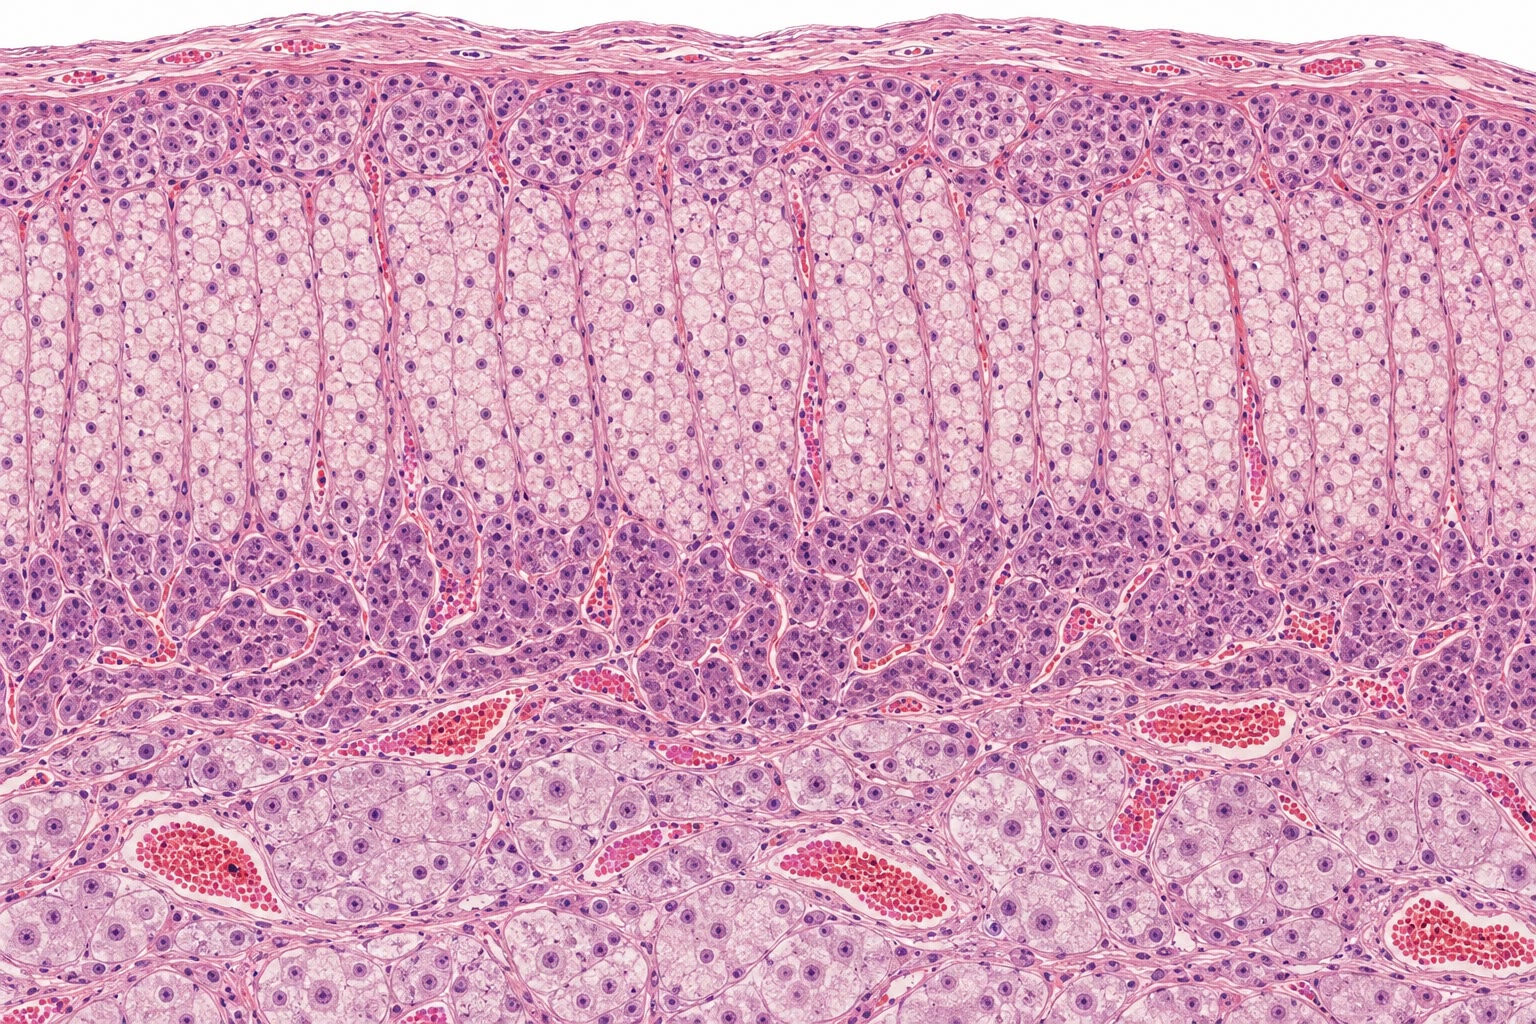
\includegraphics[width=0.5\linewidth]{images/book5/ai/b5-21-adrenal-section.jpg}\hspace{0.04\linewidth}
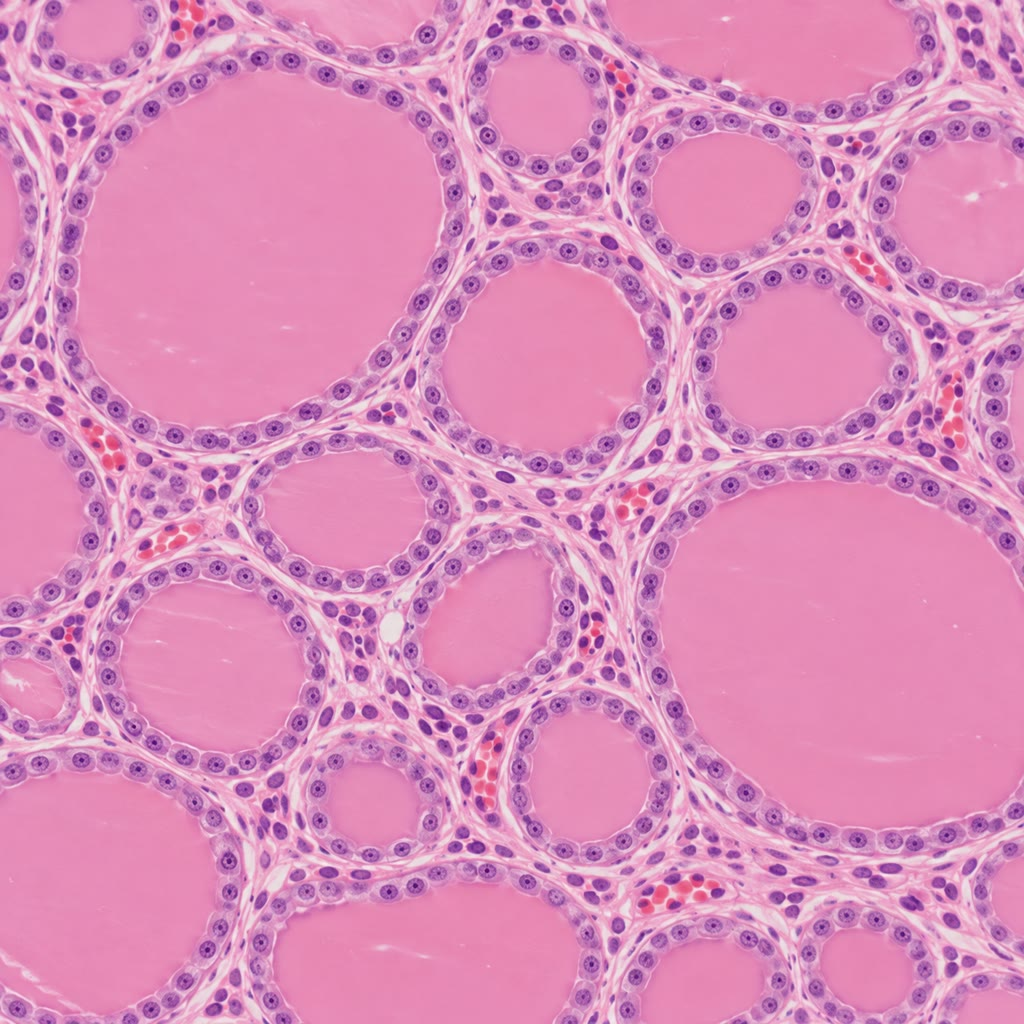
\includegraphics[width=0.36\linewidth]{images/book5/ai/b5-21-thyroid-follicles.jpg}

{\small Links: de bijnier in doorsnede --- de schors in haar drie zones
(\omterm{def:b3:renal-osmoregulation:controls}{aldosteron} het buitenst, cortisol in de brede middenzone, androgenen
het binnenst) rond een merg van adrenaline uitscheidende chromaffiene
cellen, dat naar zijn oorsprong een sympathisch \omterm{def:b3:nervous-systems:comparative}{ganglion} is. Rechts:
follikels van de schildklier, elk een bol cellen rond een voorraad
colloïd die maanden aan \omterm{def:b3:endocrinology:hormone}{hormoon} gebonden aan thyreoglobuline bevat.}
\end{omfigure}

\section{Glucose: de strakste lus}

\begin{definition}[Insuline en glucagon]\label{def:b3:endocrinology:glucose}
\index{insuline}\index{glucagon}\index{eilandje van Langerhans}\index{GLUT4}\index{diabetes mellitus}
Het bloed bevat ongeveer \qty{5}{g} glucose, bij \qty{5}{mmol/L}
(\qty{90}{mg/dL}), en het brein verbrandt er \qty{120}{g} per dag van
en kan niets anders verbranden; een maaltijd levert er in een uur
\qty{75}{g}. De \emph{eilandjes van Langerhans}, een miljoen groepjes
van enkele duizenden cellen verspreid door de alvleesklier, houden de
lus vast. $\beta$-cellen voelen de glucose door haar om te zetten: meer
glucose, meer ATP, sluiting van een ATP-gevoelig kaliumkanaal,
depolarisatie, calcium naar binnen en exocytose van \emph{insuline},
een \omterm{def:b3:endocrinology:hormone}{peptidehormoon} dat uit één voorloper wordt geknipt. Insuline zegt
spier en vet de transporter \emph{GLUT4} naar hun oppervlak te brengen
en glucose op te nemen, de lever glucose als glycogeen op te slaan en
op te houden met haar te maken, en het vet op te houden met het afgeven
van vetzuren: het is het \omterm{def:b3:endocrinology:hormone}{hormoon} van de gevoede toestand, het enige dat
de bloedglucose verlaagt. $\alpha$-cellen geven \emph{glucagon} af
wanneer de glucose daalt: de lever breekt glycogeen af en maakt nieuwe
glucose uit aminozuren en lactaat. Adrenaline, cortisol en groeihormoon
verhogen de glucose eveneens, en de overtolligheid is niet symmetrisch:
een lichaam kan zich langs vier wegen tegen een daling verweren en
langs één tegen een stijging. \emph{Diabetes mellitus} is het falen van
die ene: type 1, de auto-immuunvernietiging van de $\beta$-cellen,
vergt vanaf de eerste dag insuline; type 2, negen van de tien gevallen,
begint als ongevoeligheid van de weefsels voor insuline, die jarenlang
met meer insuline wordt beantwoord, tot de $\beta$-cellen het niet meer
bijhouden en de glucose stijgt.
\end{definition}

\begin{theorem}[De insuline--glucoselus]\label{thm:b3:endocrinology:loop}
\index{lusversterking}\index{instelpunt}\index{gedempte trilling}
Schrijf $g$ en $i$ voor de afwijkingen van de glucose en de \omterm{def:b3:endocrinology:glucose}{insuline} in
het plasma ten opzichte van hun nuchtere waarden. Glucose wordt
geklaard met een snelheid evenredig met haar eigen overmaat (de
doeltreffendheid van glucose $a$) en met de overmaat aan \omterm{def:b3:endocrinology:glucose}{insuline} (de
gevoeligheid $s$); \omterm{def:b3:endocrinology:glucose}{insuline} wordt uitgescheiden evenredig met de
overmaat aan glucose ($\beta$) en geklaard met snelheid $\gamma$; een
belasting $u$ komt binnen:
\[
\dot g = -a\,g - s\,i + u, \qquad \dot i = \beta\,g - \gamma\,i .
\]
Onder een gelijkblijvende belasting $u$ komt de glucose uit op
\[
g^{*} = \frac{u}{a}\cdot\frac{1}{1 + L}, \qquad L = \frac{s\beta}{a\gamma},
\]
zodat de terugkoppeling de verstoring die een ongeregeld lichaam zou
ondergaan deelt door $1 + L$, de \emph{\omterm{thm:b3:endocrinology:loop}{lusversterking}} plus één. Na een
bolus wordt de terugkeer bepaald door de eigenwaarden
$\lambda = -\tfrac{a + \gamma}{2} \pm \sqrt{\tfrac{(a+\gamma)^{2}}{4} - (a\gamma + s\beta)}$:
monotoon als $s\beta < (a - \gamma)^{2}/4$, en anders een \omterm{thm:b3:endocrinology:loop}{gedempte
trilling} met hoekfrequentie $\omega = \sqrt{a\gamma + s\beta -
(a+\gamma)^{2}/4}$ die uitdooft als $\mathrm{e}^{-(a+\gamma)t/2}$ --- de
glucose schiet onder haar nuchtere waarde door voordat zij uitkomt, en
dat is de milde hypoglykemie twee of drie uur na een suikerrijke
maaltijd. Ongevoeligheid voor \omterm{def:b3:endocrinology:glucose}{insuline} verlaagt $s$: de nuchtere
stationaire toestand onder de eigen afgifte van de lever stijgt, en de
lus vangt dat op met een hogere $i^{*}$ tot ook de $\beta$ van de
$\beta$-cellen daalt, en dan faalt de opvang.
\end{theorem}
\begin{proof}
Stationaire toestand: $\dot i = 0$ geeft $i^{*} = \beta g^{*}/\gamma$;
ingevuld in $\dot g = 0$: $a g^{*} + s\beta g^{*}/\gamma = u$, waaruit $g^{*} =
u/(a + s\beta/\gamma) = (u/a)/(1 + L)$. Dynamiek: de systeemmatrix is
$\begin{pmatrix} -a & -s\\ \beta & -\gamma\end{pmatrix}$, met spoor
$-(a+\gamma)$ en determinant $a\gamma + s\beta$; haar karakteristieke
vergelijking $\lambda^{2} + (a+\gamma)\lambda + (a\gamma + s\beta) = 0$ heeft
de genoemde wortels. Beide hebben een negatief reëel deel, dus is de
nuchtere toestand stabiel; de wortels zijn complex wanneer de
discriminant $(a+\gamma)^{2}
- 4(a\gamma + s\beta) = (a-\gamma)^{2} - 4s\beta$ negatief is, de
gegeven voorwaarde, en dan is $g(t) = \mathrm{e}^{-(a+\gamma)t/2}(A\cos\omega t
+ B\sin\omega t)$, dat door nul gaat. Ongevoeligheid: met $u$ de basale
afgifte van de lever en een verlaagde $s$ daalt $L$ en stijgt $g^{*}$
bij dezelfde $u$; $i^{*} = \beta g^{*}/\gamma$ stijgt mee
(hyperinsulinemie); daalt daarna $\beta$, dan daalt $L$ verder en klimt $g^{*}$ naar $u/a$.
\end{proof}

\begin{omfigure}
\begin{tikzpicture}
\begin{axis}[
  width=0.58\linewidth, height=5.6cm,
  axis x line=bottom, axis y line=left,
  xmin=0, xmax=180, ymin=40, ymax=200,
  xlabel={minuten na een glucosebolus}, ylabel={plasmaglucose (mg/dL)},
  xlabel style={font=\small, at={(axis description cs:0.5,-0.12)}, anchor=north}, ylabel style={font=\small},
  tick label style={font=\small}, xtick={0,30,60,90,120,150,180}, ytick={60,90,120,150,180},
  clip=false,
]
\addplot[very thick, omDef, smooth] coordinates {(0,190) (6,165) (12,131) (18,102) (24,84) (30,77) (36,78) (42,82) (48,86) (54,89) (60,91) (66,92) (72,91) (78,91) (84,90) (90,90) (96,90) (102,90) (108,90) (114,90) (120,90) (126,90) (132,90) (138,90) (144,90) (150,90) (156,90) (162,90) (168,90) (174,90) (180,90)};
\draw[dashed, gray] (axis cs:0,90) -- (axis cs:180,90);
\node[font=\scriptsize, gray, anchor=south east] at (axis cs:180,91) {nuchtere waarde};
\node[font=\scriptsize, omDef, anchor=west, align=left] at (axis cs:75,150) {model: $a = \qty{0.02}{min^{-1}}$, $\gamma = \qty{0.1}{min^{-1}}$,\\$s\beta = \qty{0.01}{min^{-2}}$, lusversterking $L = 5$;\\doorschot bij \qty{32}{min}, periode \qty{68}{min}};
\node[font=\scriptsize, omThm, anchor=north] at (axis cs:24,70) {doorschot};
\end{axis}
\begin{axis}[
  at={(0.6\linewidth,0)}, anchor=south west,
  width=0.33\linewidth, height=5.6cm,
  axis x line=bottom, axis y line=left,
  xmin=0, xmax=180, ymin=0, ymax=40,
  xlabel={minuten}, ylabel={insuline (mU/L)},
  xlabel style={font=\small, at={(axis description cs:0.5,-0.12)}, anchor=north}, ylabel style={font=\small},
  tick label style={font=\small}, xtick={0,60,120,180}, ytick={0,10,20,30,40},
]
\addplot[very thick, omProp, smooth] coordinates {(0,10.0) (6,30.0) (12,33.7) (18,28.5) (24,20.4) (30,13.4) (36,8.9) (42,7.1) (48,7.1) (54,7.9) (60,9.0) (66,9.8) (72,10.2) (78,10.4) (84,10.4) (90,10.2) (96,10.1) (102,10.0) (108,10.0) (114,9.9) (120,10.0) (126,10.0) (132,10.0) (138,10.0) (144,10.0) (150,10.0) (156,10.0) (162,10.0) (168,10.0) (174,10.0) (180,10.0)};
\draw[dashed, gray] (axis cs:0,10) -- (axis cs:180,10);
\end{axis}
\end{tikzpicture}

{\small De lineaire lus na een bolus die de glucose met
\qty{100}{mg/dL} verhoogt. De \omterm{def:b3:endocrinology:glucose}{insuline} piekt binnen tien minuten en de
glucose is na twintig terug op haar uitgangswaarde, waarna zij
doorschiet; een sterke terugkoppeling die via een \omterm{def:b3:endocrinology:hormone}{hormoon} met zijn
eigen klaringstijd werkt keert terug als een \omterm{thm:b3:endocrinology:loop}{gedempte trilling} en niet
als een eenvoudig verval.}
\end{omfigure}

\begin{proof}[Bewijsmateriaal]
Von Mering en Minkowski (1889) namen een hond zijn alvleesklier af en
brachten daarmee suikerziekte voort --- de vliegen die op zijn urine
afkwamen verraadden de suiker; de buizen afbinden, waarmee het
verteringsweefsel werd vernietigd maar de eilandjes werden gespaard,
deed dat niet. Banting en Best (1921) haalden, met de zuivering van
Collip, het beginsel uit de eilandjes en verlaagden de bloedsuiker van
een suikerzieke hond, en daarna die van Leonard Thompson (januari
1922). Sanger bepaalde de volgorde van \omterm{def:b3:endocrinology:glucose}{insuline} (1955), de eerste
eiwitsequentie; Yalow en Berson maten het in bloed (1959) en vonden dat
suikerzieken bij wie de ziekte op volwassen leeftijd begon er
aanvankelijk meer van hadden dan gezonden --- ongevoeligheid, geen
gebrek. De bacteriën van Genentech maakten in 1978 menselijke \omterm{def:b3:endocrinology:glucose}{insuline},
het eerste recombinante geneesmiddel.
\end{proof}

\begin{omfigure}
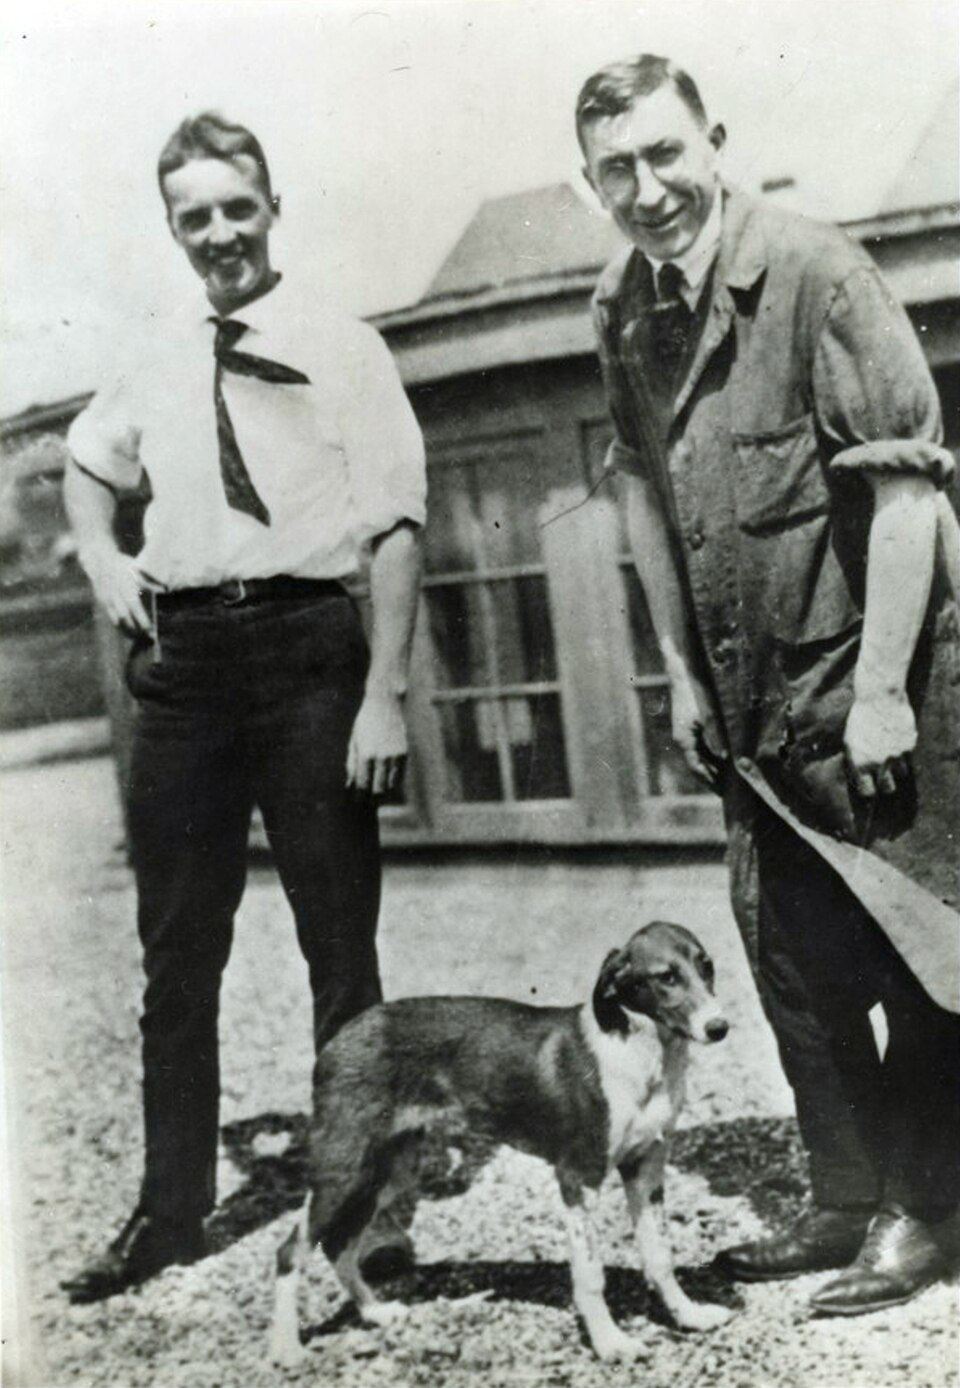
\includegraphics[width=0.42\linewidth]{images/book5/banting-best.jpg}\hspace{0.04\linewidth}
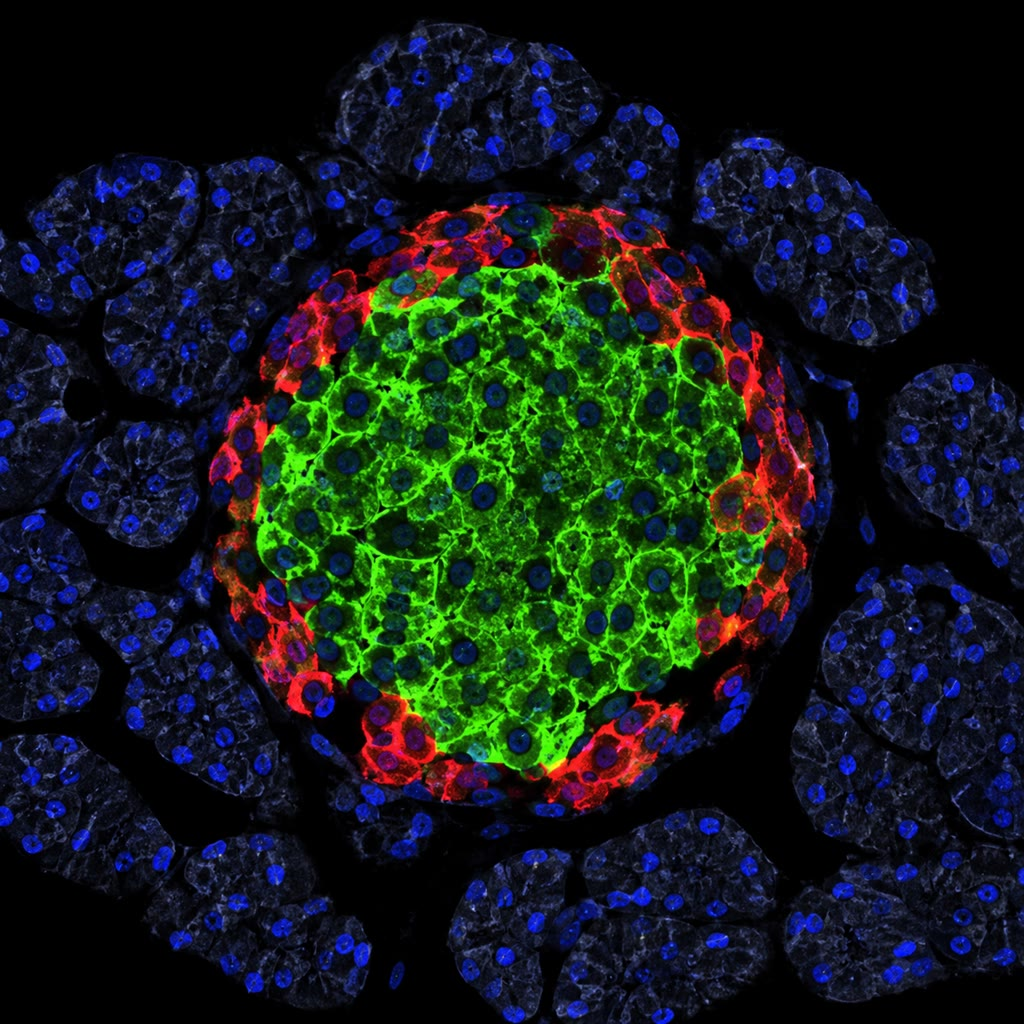
\includegraphics[width=0.42\linewidth]{images/book5/ai/b5-21-pancreatic-islet.jpg}

{\small Links: Frederick Banting en Charles Best op het dak van het
medische gebouw in Toronto, omstreeks 1924, met een van de honden van
de insulineproeven (foto in het publieke domein). Rechts: een \omterm{def:b3:endocrinology:glucose}{eilandje
van Langerhans}, met \omterm{def:b3:endocrinology:glucose}{insuline} producerende $\beta$-cellen in de kern en
glucagon-$\alpha$-cellen aan de rand, in een zee van exocriene acini.}
\end{omfigure}

\begin{method}[De glucoselus bij een patiënt aflezen]\label{met:b3:endocrinology:ogtt}
\index{glucosetolerantietest}\index{HbA1c}
(1) Nuchtere plasmaglucose: normaal onder \qty{5.6}{mmol/L}, diabetes
bij \qty{7.0}{mmol/L} of meer bij twee gelegenheden. (2) Orale
\omterm{met:b3:endocrinology:ogtt}{glucosetolerantietest}: \qty{75}{g} glucose gedronken; de plasmaglucose
na twee uur is normaal onder \qty{7.8}{mmol/L} en wijst op diabetes bij
\qty{11.1}{mmol/L} of meer --- de waarde na twee uur leest de
versterking van de lus af, de nuchtere waarde haar \omterm{thm:b3:endocrinology:loop}{instelpunt}.
(3) Geglyceerd hemoglobine, \emph{HbA1c}: glucose hecht zich
onomkeerbaar aan hemoglobine met een snelheid evenredig aan haar
concentratie, en rode cellen leven 120 dagen, zodat de geglyceerde
fractie de gemiddelde glucose van de afgelopen drie maanden integreert
zonder dat er gevast hoeft te worden --- normaal onder \qty{5.7}{\%},
diabetes vanaf \qty{6.5}{\%}. (4) Om ongevoeligheid van gebrek te
scheiden: meet de \omterm{def:b3:endocrinology:glucose}{insuline} (of haar bijproduct C-peptide) ernaast; hoge
\omterm{def:b3:endocrinology:glucose}{insuline} bij hoge glucose is ongevoeligheid, afwezig C-peptide is
type~1.
\end{method}

\section{Calcium, en de klok}

\begin{definition}[Calciumhomeostase]\label{def:b3:endocrinology:calcium}
\index{bijschildklierhormoon}\index{calcitriol}\index{vitamine D}\index{osteoporose}
Geïoniseerd calcium in het plasma wordt binnen enkele procenten op
\qty{1.2}{mmol/L} gehouden, omdat het de prikkelbaarheid van elke zenuw
en elke spier bepaalt: te laag en zij vuren spontaan (tetanie), te hoog
en zij worden traag. De vier bijschildklieren voelen het met een
receptor aan het oppervlak en scheiden \emph{bijschildklierhormoon}
(PTH) uit langs een steile omgekeerde sigmoïde: PTH mobiliseert calcium
uit het bot, laat de nier het terugnemen en fosfaat uitscheiden, en
activeert \emph{vitamine D} --- in de huid door ultraviolet licht
gemaakt of gegeten, gehydroxyleerd in de lever en daarna in de nier tot
\emph{calcitriol} --- dat de darm calcium doet opnemen. Het bot is het
reservoir, een kilogram calcium, dat voortdurend door osteoclasten en
osteoblasten wordt verbouwd onder PTH, calcitriol, oestrogeen en
belasting. Gebrek aan vitamine D geeft rachitis bij kinderen en zachte
botten bij volwassenen; de daling van het oestrogeen bij de overgang
kantelt de verbouwing naar afbraak en geeft \emph{osteoporose}; een
adenoom van een bijschildklier verhoogt het calcium, lost het bot op en
vormt nierstenen --- ``botten, stenen, kreunen en klagen.''
\end{definition}

\begin{definition}[De circadiane klok]\label{def:b3:endocrinology:clock}
\index{circadiane klok}\index{suprachiasmatische kern}\index{klokgenen}\index{melatonine}\index{zeitgeber}
Vrijwel elke cel draagt een \emph{circadiane klok}: een lus van
transcriptie en translatie waarin de eiwitten CLOCK en BMAL1 de genen
\emph{Per} en \emph{Cry} aanzetten, wier eiwitten zich ophopen, na een
vertraging van uren de kern binnengaan en hun eigen transcriptie
onderdrukken, en daarna worden afgebroken, waarmee de onderdrukking
wordt opgeheven --- één cyclus in ongeveer vierentwintig uur, bepaald
door de snelheden van de vertraging en de afbraak. De klokken van het
lichaam worden gelijkgezet door een hoofdklok van twintigduizend
neuronen in de \emph{suprachiasmatische kern} van de \omterm{def:b3:endocrinology:axes}{hypothalamus}, die
zelf door licht wordt gezet via een eigen klasse ganglioncellen van het
\omterm{def:b3:sensory-systems:retina}{netvlies} (die melanopsine bevatten, niet de pigmenten van de \omterm{def:b3:sensory-systems:retina}{staafjes}
of de \omterm{def:b3:sensory-systems:retina}{kegeltjes}), en die het lichaam de nacht aanzegt met het
\emph{melatonine} van de pijnappelklier, dat alleen in het donker wordt
afgegeven. De klok plant cortisol vóór het ontwaken, de laagste
lichaamstemperatuur om vier uur 's nachts, groeihormoon in de eerste
slaap, en een hogere gevoeligheid voor \omterm{def:b3:endocrinology:glucose}{insuline} in de ochtend; voedsel,
beweging en temperatuur zijn ondergeschikte \emph{zeitgebers} die de
perifere klokken van de centrale kunnen wegtrekken, en dat is de
malaise van de ploegenwerker en van de jetlag --- een leverklok op de
ene tijd en een brein op de andere.
\end{definition}

\begin{proof}[Bewijsmateriaal]
Konopka en Benzer (1971) zochten in gemuteerde vliegen naar veranderde
ritmen van het uitkomen en vonden drie allelen van één gen,
\emph{period}: een korte dag (19 h), een lange dag (29 h) en in het
geheel geen ritme --- een klok met een genetische periode. Hardin, Hall
en Rosbash (1990) vonden dat het mRNA en het eiwit van \emph{period}
oscilleren met een vertraging ertussen, en dat het eiwit zijn eigen gen
onderdrukt: de lus. Ralph en Menaker (1990) verplantten de
\omterm{def:b3:endocrinology:clock}{suprachiasmatische kern} van een gemuteerde hamster met een ritme van 20
uur in een normale hamster wier eigen kern was vernietigd: de ontvanger
draaide op 20 uur --- de periode hoorde bij het verplante weefsel. Bij
mensen die zonder tijdsaanwijzingen in een bunker werden gehouden liep
het ritme vrij op iets meer dan 24 uur; fel licht in de avond
vertraagde het, in de ochtend vervroegde het.
\end{proof}

\begin{omfigure}
\begin{tikzpicture}[every node/.style={font=\scriptsize}, >=stealth]
  \node[draw, thick, rounded corners, fill=omDef!20, align=center] (cb) at (0,1.6) {CLOCK--BMAL1\\activatoren};
  \node[draw, thick, rounded corners, fill=omProp!25, align=center] (pc) at (3.6,1.6) {\emph{Per}, \emph{Cry}\\afgeschreven};
  \node[draw, thick, rounded corners, fill=omThm!20, align=center] (pr) at (3.6,-0.4) {eiwitten PER en CRY\\hopen zich op, dimeriseren};
  \node[draw, thick, rounded corners, fill=omMeth!25, align=center] (nu) at (0,-0.4) {gaan na uren\\de kern in};
  \draw[->, thick] (cb) -- (pc) node[midway, above, font=\tiny] {activeren};
  \draw[->, thick] (pc) -- (pr) node[midway, right, font=\tiny] {translatie, vertraging};
  \draw[->, thick] (pr) -- (nu);
  \draw[-|, thick, omThm] (nu) -- (cb) node[midway, left, font=\tiny, omThm, align=right] {onderdrukken\\hun eigen\\activatoren};
  \draw[->, thick, gray] (nu.south) -- ++(0,-0.5) node[below, font=\tiny, gray, align=center] {afgebroken: de onderdrukking valt weg,\\de cyclus begint opnieuw $\approx$ \qty{24}{h}};
  % right: daily profile
  \begin{scope}[shift={(7.2,-1.6)}]
    \draw[->] (0,0) -- (5.6,0) node[right, font=\tiny] {uur};
    \draw[->] (0,0) -- (0,3.4);
    \foreach \x/\l in {0/0, 1.4/6, 2.8/12, 4.2/18, 5.6/24} { \draw (\x,0) -- (\x,-0.08) node[below, font=\tiny] {\l}; }
    \fill[gray!25] (0,0) rectangle (1.4,3.4); \fill[gray!25] (5.1,0) rectangle (5.6,3.4);
    \node[font=\tiny, gray!60!black] at (0.7,3.2) {nacht};
    \draw[very thick, omMeth!70!black, domain=0:5.6, samples=60, smooth, variable=\x] plot (\x, {1.6 + 1.2*cos(deg(2*3.1416*(\x-1.9)/5.6))});
    \node[font=\tiny, omMeth!70!black] at (3.1,3.1) {cortisol: piek om 8 uur};
    \draw[very thick, omDef, domain=0:5.6, samples=60, smooth, variable=\x] plot (\x, {0.9 + 0.7*cos(deg(2*3.1416*(\x-0.7)/5.6))});
    \node[font=\tiny, omDef] at (2.7,0.18) {melatonine: alleen 's nachts};
  \end{scope}
\end{tikzpicture}

{\small Links: de kern van de moleculaire klok, een negatieve
terugkoppelingslus met een vertraging van uren, wat een lus nodig heeft
om te oscilleren in plaats van tot rust te komen. Rechts: twee \omterm{def:b3:endocrinology:hormone}{hormonen}
die zij inroostert --- cortisol dat vóór de dageraad stijgt om de dag
voor te bereiden, \omterm{def:b3:endocrinology:clock}{melatonine} dat de nacht markeert.}
\end{omfigure}

\begin{remark}[Homeostase als regeling]\label{rem:b3:endocrinology:control}
Elke lus in dit hoofdstuk heeft dezelfde onderdelen: een voeler (de
stofwisseling van de $\beta$-cel, de calciumreceptor van de
bijschildklier, de schildklierhormoonreceptor van de \omterm{def:b3:endocrinology:axes}{hypofyse}), een
regelaar die met een \omterm{thm:b3:endocrinology:loop}{instelpunt} vergelijkt, een uitvoerend \omterm{def:b3:endocrinology:hormone}{hormoon} met
zijn eigen halveringstijd, en een terugkoppeling die de fout met een
factor $1 + L$ verkleint maar nooit tot nul. Wat verschilt is de
tijdschaal --- seconden voor adrenaline, een uur voor \omterm{def:b3:endocrinology:glucose}{insuline}, dagen
voor thyroxine, een leven voor bot --- en de prijs van het compromis:
een snelle lus met een vertraagde uitvoerder oscilleert, een trage lus
laat een verstoring voortduren. De kliniek ziet de lussen van buitenaf,
door de paren die de terugkoppeling koppelt: een hoge TSH bij een laag
T$_{4}$ is een falende klier, een hoge TSH bij een hoog T$_{4}$ een
falende \omterm{def:b3:endocrinology:axes}{hypofyse}; een hoge \omterm{def:b3:endocrinology:glucose}{insuline} bij een hoge glucose is
ongevoeligheid, een lage \omterm{def:b3:endocrinology:glucose}{insuline} bij een hoge glucose is vernietiging.
Om een hormoonspiegel te lezen moet men altijd vragen wat de
bevelvoerder ervan deed.
\end{remark}

\section{Opgaven}

\begin{exercise}[$\star$]\label{exo:b3:endocrinology:1}
Deel \omterm{def:b3:endocrinology:glucose}{insuline}, cortisol, adrenaline, thyroxine en vasopressine in naar
chemie, plaats van de receptor, snelheid van werking en halveringstijd.
\end{exercise}

\begin{exercise}[$\star$]\label{exo:b3:endocrinology:2}
Teken de schildklieras met haar terugkoppeling en voorspel TSH en
T$_{4}$ bij: een vernietigde schildklier; een \omterm{def:b3:cancer-biology:hallmarks}{tumor} van de \omterm{def:b3:endocrinology:axes}{hypofyse} die
TSH uitscheidt; een patiënt die te veel thyroxine slikt; jodiumgebrek.
\end{exercise}

\begin{exercise}[$\star$]\label{exo:b3:endocrinology:3}
Waarom heeft een lichaam vier \omterm{def:b3:endocrinology:hormone}{hormonen} die de bloedglucose verhogen en
maar één dat haar verlaagt? Wat voorspelt dat over de betrekkelijke
gevaren van te veel en te weinig \omterm{def:b3:endocrinology:glucose}{insuline}?
\end{exercise}

\begin{exercise}[$\star$]\label{exo:b3:endocrinology:4}
Wat is een \omterm{def:b3:endocrinology:clock}{zeitgeber}? Geef er drie, zeg welke de hoofdklok gebruikt, en
leg uit wat er gebeurt met een reiziger die acht tijdzones oversteekt.
\end{exercise}

\begin{exercise}[$\star\star$]\label{exo:b3:endocrinology:5}
Een cel heeft \num{20000} receptoren met $K_{d} = \qty{1}{nM}$ en
antwoordt maximaal wanneer er \num{500} bezet zijn. Bepaal de
EC$_{50}$. Na een week met veel \omterm{def:b3:endocrinology:hormone}{hormoon} heeft de cel nog \num{2000}
receptoren: nieuwe EC$_{50}$? Duid dit voor de ongevoeligheid voor
\omterm{def:b3:endocrinology:glucose}{insuline}.
\end{exercise}

\begin{exercise}[$\star\star$]\label{exo:b3:endocrinology:6}
Bereken met $\kappa = \qty{0.46}{L/pmol}$ en een normale TSH van
\qty{1.5}{mU/L} bij een vrij T$_{4}$ van \qty{15}{pmol/L} de TSH
wanneer T$_{4}$ gelijk is aan $13$, $11$, $9$ en \qty{25}{pmol/L}. Bij
welke daarvan zou T$_{4}$ nog binnen een referentiegebied van
\qtyrange{10}{20}{pmol/L} liggen terwijl de TSH buiten
\qtyrange{0.4}{4}{mU/L} valt?
\end{exercise}

\begin{exercise}[$\star\star$]\label{exo:b3:endocrinology:7}
Bereken in de lus van \cref{thm:b3:endocrinology:loop} met $a = \qty{0.02}{min^{-1}}$,
$\gamma = \qty{0.1}{min^{-1}}$, $\beta = \qty{0.05}{mU\,L^{-1}\,min^{-1}}$
per mg/dL en $s = \qty{0.2}{mg\,dL^{-1}\,min^{-1}}$ per mU/L de
\omterm{thm:b3:endocrinology:loop}{lusversterking}, de stationaire overmaat aan glucose onder een
gelijkblijvende belasting van \qty{2}{mg/dL/min}, dezelfde zonder
terugkoppeling, en de stationaire overmaat aan \omterm{def:b3:endocrinology:glucose}{insuline}.
\end{exercise}

\begin{exercise}[$\star\star$]\label{exo:b3:endocrinology:8}
Dezelfde parameters: is de terugkeer na een bolus oscillerend? Bereken
de periode en de tijd waarin de amplitude met een factor $\mathrm{e}$
daalt. Halveer nu $s$ (ongevoeligheid voor \omterm{def:b3:endocrinology:glucose}{insuline}): bereken beide
opnieuw en de nieuwe \omterm{thm:b3:endocrinology:loop}{lusversterking}.
\end{exercise}

\begin{exercise}[$\star\star$]\label{exo:b3:endocrinology:9}
De halveringstijd van cortisol is \qty{80}{min}. Een patiënt die een
jaar lang dagelijks \qty{40}{mg} prednisolon gebruikt stopt abrupt. Leg
laag voor laag uit waarom hij drie dagen later bij een lichte
besmetting kan instorten, en wat de as zou tonen als zij werd gemeten
(ACTH, cortisol, antwoord op ingespoten ACTH).
\end{exercise}

\begin{exercise}[$\star\star\star$]\label{exo:b3:endocrinology:10}
Laat zien dat een \omterm{def:b3:endocrinology:axes}{negatieve terugkoppeling} met één variabele, $\dot x = f(x)$
met $f' < 0$, niet kan oscilleren terwijl de lus met twee
variabelen uit de stelling dat wel kan, en leg in woorden uit waarom de
klok een vertraging van uren tussen transcriptie en onderdrukking nodig
heeft om een periode van 24 uur voort te brengen. Wat zou er met de
periode gebeuren als PER tweemaal zo snel werd afgebroken?
\end{exercise}

\begin{exercise}[$\star\star\star$]\label{exo:b3:endocrinology:11}
Het \omterm{def:b3:endocrinology:calcium}{bijschildklierhormoon} volgt $\text{PTH} = P_{\max}/(1 +
\mathrm{e}^{k(\text{Ca} - \text{Ca}_{0})})$ met $\text{Ca}_{0} =
\qty{1.2}{mmol/L}$ en $k = \qty{20}{L/mmol}$. Bereken PTH als fractie
van het maximum bij Ca $= 1.10$, $1.15$, $1.20$, $1.25$ en \qty{1.30}{mmol/L},
de helling in het \omterm{thm:b3:endocrinology:loop}{instelpunt}, en leg uit waarom zulke steilheid voor
calcium gewenst is maar voor glucose gevaarlijk zou zijn.
\end{exercise}

\begin{exercise}[$\star\star\star$]\label{exo:b3:endocrinology:12}
Glucose hecht zich met een snelheid $k\,G$ per tijdseenheid aan
hemoglobine, met $k$ zo dat een gemiddelde glucose van \qty{5.5}{mmol/L}
over de 120 dagen van het leven van een rode cel \qty{5}{\%} glycering
geeft. Leid HbA1c af als functie van de gemiddelde glucose, geef de
waarde bij \qty{10}{mmol/L}, en leg uit waarom een patiënt met een
hemolytische bloedarmoede (rode cellen die 60 dagen leven) een
misleidend laag HbA1c heeft.
\end{exercise}

\section{Vraagstuk: de suiker in het bloed}

\begin{problem}[{Weekendvraagstuk --- een \omterm{met:b3:endocrinology:ogtt}{glucosetolerantietest} gelezen
door de lineaire insuline--glucoselus: de verdeling van een dosis van
\qty{75}{g}, de \omterm{thm:b3:endocrinology:loop}{lusversterking} en de gedempte terugkeer, wat
ongevoeligheid en het falen van de $\beta$-cellen met het nuchtere
\omterm{thm:b3:endocrinology:loop}{instelpunt} doen, een diagnose uit de getallen, en de schildklieras
ernaast, eindigend bij de \omterm{thm:b3:endocrinology:loop}{lusversterking}, de terugkeertijd en de
nuchtere glucose van de falende lus}]
\label{pb:b3:endocrinology:1}
Gegevens: een gezonde volwassene, verdelingsvolume voor glucose
\qty{15}{L}, nuchtere glucose \qty{90}{mg/dL} (\qty{5}{mmol/L}),
nuchtere \omterm{def:b3:endocrinology:glucose}{insuline} \qty{10}{mU/L}. Parameters van de lus: $a = \qty{0.02}{min^{-1}}$, $\gamma =
\qty{0.1}{min^{-1}}$, $\beta = 0.05$ (mU/L per min per mg/dL), $s = 0.2$
(mg/dL per min per mU/L). Basale glucoseafgifte van de lever $u_{0} =
\qty{2}{mg/dL/min}$ (in de nuchtere toestand al in evenwicht met de
nuchtere afvoer). Een orale dosis van \qty{75}{g} wordt in een uur
opgenomen. Schildklier: $\text{TSH} = 1.5\,\mathrm{e}^{-0.46(T_{4} - 15)}$ mU/L.
Molaire massa van glucose \qty{180}{g/mol}.

\medskip
\noindent\textbf{Deel I --- De dosis.}
\begin{enumerate}
  \item Druk de nuchtere glucose uit in mmol/L en controleer de
        omrekening uit mg/dL. Hoeveel gram glucose bevindt zich nuchter
        in het verdelingsvolume?
  \item Als de hele \qty{75}{g} in één keer in \qty{15}{L} zou
        verschijnen, met hoeveel zou de glucose dan stijgen (mg/dL en
        mmol/L)? Waarom blijft de werkelijke piek, ongeveer
        \qty{60}{mg/dL} boven nuchter, daar zo ver bij achter?
  \item Met welke snelheid in mg/dL per minuut komt de dosis binnen als
        zij over \qty{60}{min} wordt opgenomen? Vergelijk met $u_{0}$.
  \item Zonder enig insuline-antwoord ($s = 0$) zou de glucose voldoen aan $\dot
        g = -a g + u$. Stationaire overmaat bij het opnametempo, en de
        tijdconstante van de nadering. Waar zou de glucose na een uur
        staan?
  \item Bereken met de lus $L$ en de stationaire overmaat bij hetzelfde
        tempo. Vergelijk met vraag~4.
  \item Leg uit waarom het brein aan beide kanten wordt beschermd: wat
        het nodig heeft, en wat te veel glucose in jaren met de weefsels doet.
\end{enumerate}

\medskip
\noindent\textbf{Deel II --- De terugkeer.}
\begin{enumerate}[resume]
  \item Schrijf de karakteristieke vergelijking van de lus op en
        bereken het spoor, de determinant en de discriminant.
  \item Bereken $\omega$ en de periode van de \omterm{thm:b3:endocrinology:loop}{gedempte trilling}, en de
        vervaltijd $2/(a + \gamma)$.
  \item Uitgaande van een overmaat van \qty{100}{mg/dL} met de \omterm{def:b3:endocrinology:glucose}{insuline}
        op haar nuchtere waarde luidt de oplossing $g(t) = 100\,\mathrm{e}^{-0.06t}
        (\cos\omega t + c\sin\omega t)$. Bepaal $c$ uit $\dot g(0) = -a\cdot
        100$.
  \item Wanneer keert de glucose voor het eerst terug naar nuchter (de
        eerste nulwaarde van $g$)? Schat het doorschot bij het eerste minimum.
  \item \omterm{def:b3:endocrinology:glucose}{Insuline}: $i(t)$ heeft dezelfde e-macht en frequentie.
        Beredeneer uit $\dot i = \beta g - \gamma i$ dat haar piek komt
        nadat de glucose is beginnen te dalen en voordat de glucose
        nuchter bereikt.
  \item Waarom toont een echte tolerantietest, met opname over een uur
        in plaats van een bolus, een piek na 30--60 minuten en een
        terugkeer binnen twee uur, en maar een milde dip na drie?
\end{enumerate}

\medskip
\noindent\textbf{Deel III --- Wanneer de lus faalt.}
\begin{enumerate}[resume]
  \item Ongevoeligheid voor \omterm{def:b3:endocrinology:glucose}{insuline} halveert $s$. Nieuwe $L$? De
        $u_{0}$ van de lever wordt nu beantwoord door een nieuwe
        nuchtere stationaire toestand: bepaal met $g^{*} = (u_{0}/a)/(1
        + L)$ als overmaat boven een geïdealiseerde ongeregelde
        uitgangswaarde met hoeveel de nuchtere glucose stijgt ten
        opzichte van de gezonde toestand (bereken beide waarden van
        $g^{*}$ en trek ze af).
  \item Nuchtere \omterm{def:b3:endocrinology:glucose}{insuline} in de ongevoelige toestand: bereken $i^{*} = \beta
        g^{*}/\gamma$ voor beide toestanden en de verhouding. Hoe heet
        dat in de kliniek?
  \item Nu falen de $\beta$-cellen: ook $\beta$ daalt tot een vijfde.
        Nieuwe $L$, nieuwe nuchtere overmaat. Reken om naar mmol/L en
        vergelijk met de diabetesdrempel van \qty{7}{mmol/L}.
  \item Is de terugkeer in de toestand van vraag~15 nog oscillerend?
        Bereken de discriminant en de tijdconstante van de traagste
        mode.
  \item Een patiënt heeft een nuchtere glucose van \qty{8}{mmol/L}, een
        nuchtere \omterm{def:b3:endocrinology:glucose}{insuline} van \qty{30}{mU/L} en een waarde na twee uur
        van \qty{13}{mmol/L}. Stel type en mechanisme vast uit de paren.
  \item Een ander heeft een nuchtere glucose van \qty{15}{mmol/L}, geen
        aantoonbaar C-peptide, en is in twee maanden \qty{8}{kg}
        afgevallen. Stel de diagnose, en verklaar het gewichtsverlies
        uit wat de weefsels zonder \omterm{def:b3:endocrinology:glucose}{insuline} doen.
  \item HbA1c: als de gemiddelde glucose van de eerste patiënt
        \qty{9}{mmol/L} is, en \qty{5.5}{mmol/L} \qty{5}{\%} geeft,
        schat dan zijn HbA1c in de veronderstelling van evenredigheid.
\end{enumerate}

\medskip
\noindent\textbf{Deel IV --- De klier ernaast.}
\begin{enumerate}[resume]
  \item Het vrije T$_{4}$ is \qty{12}{pmol/L}. Bereken de TSH. Ligt het
        T$_{4}$ in het gebied \qtyrange{10}{20}{pmol/L}? Ligt de TSH in
        \qtyrange{0.4}{4}{mU/L}? Hoe heet die toestand?
  \item T$_{4}$ is \qty{7}{pmol/L}: TSH? Een patiënt met dit T$_{4}$
        maar met een TSH van \qty{0.3}{mU/L}: waar zit de laesie?
  \item De halveringstijd van thyroxine is \qty{7}{dagen}. Een patiënt
        die het als vervanging gebruikt vergeet een week lang zijn
        tabletten. Tot welke fractie daalt de spiegel, en waarom is die
        vergeten week minder gevaarlijk dan een vergeten dag
        cortisolvervanging?
  \item De ziekte van Graves: een \omterm{def:b3:adaptive-immunity:antibody}{antilichaam} bezet de TSH-receptor.
        Voorspel T$_{4}$, TSH, en het effect van het log-lineaire
        verband op de gemeten TSH.
  \item Leg in één alinea uit waarom een hormoonspiegel zonder de
        spiegel van zijn bevelvoerder betekenisloos is, aan de hand van
        de vier paren uit de laatste opmerking van het hoofdstuk.
  \item Vat samen: de \omterm{thm:b3:endocrinology:loop}{lusversterking} bij de gezonde (vraag~5), de
        periode en de vervaltijd van de terugkeer (vraag~8), en de
        nuchtere glucose van de falende lus (vraag~15).
\end{enumerate}
\end{problem}
